\chapter{Introduction}
In this thesis methods to improve the stability of the electron gun of the \gls{flute} accelerator are studied.

\Gls{flute} is a \gls{linac} based \gls{thz} photon source currently under commission aiming to be a source of high field THz pulses in the femtosecond range, provide a test facility for accelerator research and an injection device for \gls{cstart} (see \cite{SchaeferHaererPapash2019_1000091183}) in the future. \cite{Naknaimueang:2011zz}

The design aims for a final electron energy of \SI{41}{\MeV} and bunch charges of \SIrange{1}{3000}{\pico\coulomb} with lengths of \SIrange{1}{300}{\fs}. The bunches are emitted with a repetition frequency of up to \SI{10}{\hertz}. \cite{Malygin2018}

\autoref{fig:fluteEgun-flutePaper} shows the finished accelerator schematically. The accelerator mainly consists of the low energy section, the \gls{linac} and the four-dipole bunch compressor.\\
Along with several diagnostic devices, the low energy section contains the electron gun that pre-accelerates electrons to \SI{7}{\MeV}. The electrons are generated at the cathode inside the electron photo-electrically through stimulation with \gls{uv} radiation (\SI{270}{\nm}) generated by a Ti:Sa laser. After that a solenoid is used to focus the electron beam in the horizontal and vertical plane for injection into the \gls{linac} section. The \gls{linac}, a 156-cell traveling wave structure, is then used to accelerate the electrons to \SI{41}{\MeV}. With a setup of four dipole magnets, the bunches are compressed longitudinally before the last dipole is used to generate \gls{csr} and \gls{cer} for \gls{thz} experiments. \cite{Nasse:IPAC13-WEPWA010}

At the time of writing, the low energy section is fully operational and at the end a Faraday cup is installed to measure the bunch charges.

\begin{figure}[tb]
	\centering
	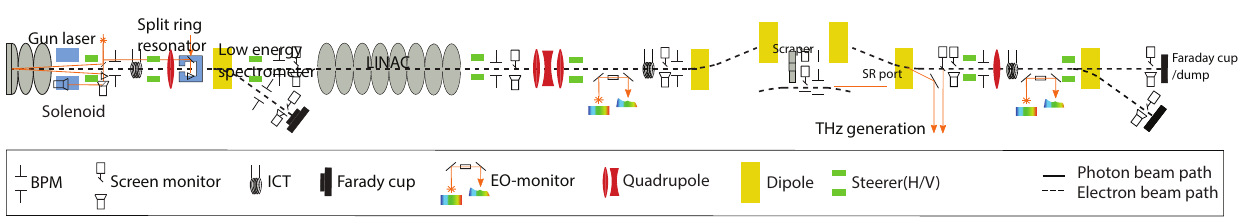
\includegraphics[width=\textwidth]{chap/StabilityOfTheElectronGun/img/flutePaper.png}
	\caption{Schematic of the finished accelerator showing all installed and planned components \cite{Yan2018}}
	\label{fig:fluteEgun-flutePaper}
\end{figure}

Scientific experiments, such as \gls{thz} spectroscopy, rely on a known and stable wavelength of the \gls{thz} radiation. As the \gls{thz} radiation is emitted from a metal target by the photo effect after being hit by the electron bunches, the wavelength and the wavelength stability of the \gls{thz} photons depend on the energy and the energy stability of the electrons.
Also as \gls{flute} being a test facility, adding and changing out components, possibly developed by other research institutes, is a common routine. To ensure compatibility among these components, reliable beam parameters at the interfaces between them are necessary. These parameters include the beams position in the $x$- and $y$-direction, the beam steering angle, the electron energy and the charge of the bunch and its dimensions. Since focusing and steering of the beam is done with electromagnets, it is also effected by the electron energy, as the deflection of an electron in a magnetic field is a function of its velocity, so ultimately its energy.

Besides depending on the \gls{uv} pulses hitting the cathode, there is also a strong dependence of the electron energies on the geometrical, electrical and thermal characteristics of the electron gun and its \gls{rf} power supply. These characteristics are not independent of each other and changes to them can have a multitude of intrinsic or extrinsic causes.

To improve the stability of the electron energy, in this thesis these causes are analyzed and measures against them or their effects are developed.

